\section{Introduction}
\subsection{Contexte}
\begin{frame}
    \frametitle{\color{white}Contexte}
    \begin{block}{Qu'est ce que OpenPGP ?}
    	\begin{itemize}
         \item Format de cryptographie normalisé dans la RFC 4880.
         \item Décrit le format des messages adapté aux outils permettant l’envoi ou le stockage sécurisés de message.
       \end{itemize} 
    \end{block}
    \begin{block}{Qu'est ce que GnuPG ?}
      \begin{itemize}
        \item GnuPG (GNU Privacy Guard) est un de ces outils.
        \item Basé sur le logiciel PGP 
        \item Utilise un système hybride cryptographie symétrique/asymétrique.
        \item Permet l'envoi de messages chiffrés et/ou signés.
        \item Les utilisateurs doivent s'envoyer leur clé publique.
      \end{itemize}
    \end{block}
\end{frame}

\subsection{Équipe}
\begin{frame}
    \frametitle{\color{white}Équipe}
  \begin{center}
    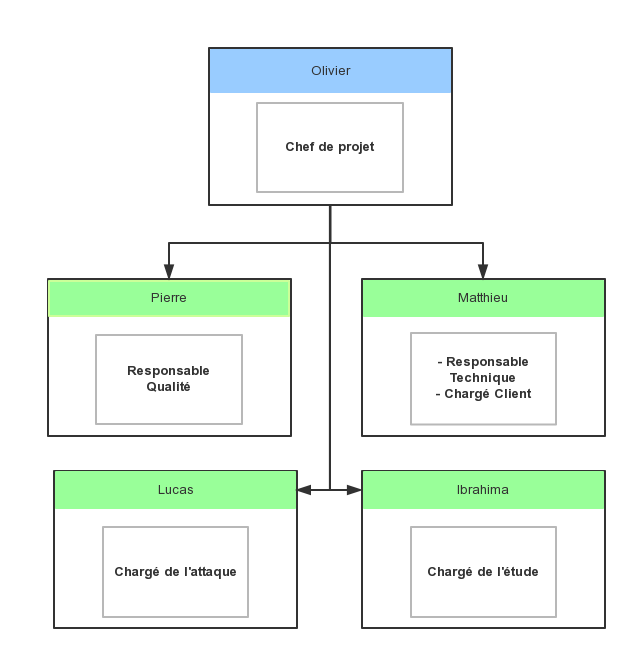
\includegraphics[scale=0.30]{guipgteam.png}
  \end{center}
\end{frame}
